\documentclass[conference, a4paper]{IEEEtran}

\usepackage{graphicx}

% used for flow charts
\usepackage{pgf}
\usepackage{tikz}
\usepackage{tikz-qtree}
\usepackage{reotex}

% package url is used when citing a website
\usepackage{url}

\usepackage{amssymb}
\usepackage{amsmath}
\usepackage{cite}
\usepackage[normalem]{ulem}
% for a smile-face character
\usepackage{wasysym}
% listing for codes
\usepackage{listings}
% listing for golang
% NOTE listings-golang.sty is required
\usepackage{listings-golang}
% to support flow graphs
\usepackage{textcomp}
% highlight in tables
\usepackage{xcolor}
\usepackage{colortbl}
% used to encode algorithms
\usepackage[linesnumbered, ruled, vlined]{algorithm2e}
\usepackage{array}

% positioning is used for below lef = of
\usetikzlibrary{shapes,shadows,arrows,automata,positioning}
% some tikz-styles on reo channels, not required in papers that have nothing to do with Reo

% finally no todos should exist in this draft
% \usepackage[textsize=tiny]{todonotes}

% -------------------------------------- configurations -----------------------------------------
% declaration of environments
\newtheorem{theorem}{Theorem}
\newtheorem{definition}{Definition}
\newtheorem{example}{Example}

% personal characters
\newcommand{\rblock}[0]{\circleddash}
\newcommand{\rread}[0]{\rhd}
\newcommand{\rnoread}[0]{\oslash}
\newcommand{\smap}[1]{[{#1}]}
\newcommand{\rempty}[0]{\varnothing}

\newcommand{\OUT}[0]{\mbox{OUT}}
\newcommand{\IN}[0]{\mbox{IN}}

% style of source code environment listings
\lstset{basicstyle=\footnotesize\ttfamily,breaklines=true, frame=shadowbox}
\lstset{numbers=left}
\lstset{xleftmargin=2em, xrightmargin=2em}
\lstset{language=Golang}

% --------------------------------------- information -------------------------------------------
\title{Active Learning from Blackbox to Timed Connectors}
\author{
\IEEEauthorblockN{Yi Li\IEEEauthorrefmark{1}, Yiwu Wang\IEEEauthorrefmark{1} and Meng Sun\IEEEauthorrefmark{1}}
\IEEEauthorblockA{
\IEEEauthorrefmark{1}Department of Informatics, School of Mathematical Sciences, Peking University,
Beijing, China\\
liyi\_math@pku.edu.cn, yiwuwang@126.com, summeng@math.pku.edu.cn
}
}

\begin{document}
\maketitle 
\begin{abstract}
  Coordination models and languages play a key role in formally specifying the communication and
  interaction among different components in large-scale distributed and concurrent systems. In this
  paper, we propose an active learning framework to extract timed connector models from black-box
  system implementation. 
  We first introduce parameterized Mealy machine(PMM) as an operational semantic
  model for channel-based coordination language Reo. PMM serves as a bridge
  between Reo connectors and Mealy machines. With the product operator, complex connectors can be
  constructed by joining basic channels and the PMM of connectors can be transformed into Mealy
  machines. Moreover, we adapt L*, a well-known learning algorithm, to timed connectors (in the form
  of Mealy machines). The new algorithm has shown its efficiency in multiple case studies. 
  This framework has been implemented in \texttt{Golang}.
\end{abstract}

\begin{IEEEkeywords}
  Active Learning, Coordination Languages, Timed Connectors
\end{IEEEkeywords}

\section{Introduction} 

Distributed real-time embedded systems (DRES) are reforming our lives with the
Internet of Things(IoT), wherein individual components are composed via \emph{connectors} 
to build systems. Such systems could be distributed logically or physically, which
makes coordination processes even more complicated. In this case, we need to specify the coordination
processes with \emph{coordination languages}, such that formal techniques can be applied to
guarantee their reliability.

\emph{Timed Reo} is a real-time extension of the coordination language \emph{Reo}, which can be used
to describe the coordination process in DRES clearly and intuitively. Different formal
semantics have been proposed to specify the behavior of timed Reo.
For example, an operational semantics based on \emph{timed constraint automata} was raised by Baier et
al.\cite{DBLP:conf/sefm/ArbabBBR04}, where a variant of LTL was also proposed to describe the
properties of timed connectors.
In \cite{DBLP:conf/tase/Meng12}, a UTP design model was proposed to specify the behavior of timed
connectors.. 

Formal verification and validation techniques have also been proved applicable for timed connectors, 
e.g. a comformance testing framework on timed connectors has been proposed in \cite{DBLP:conf/tase/LiCWS15}.
A SAT-based bounded model checking approach was adapted in \cite{DBLP:journals/scp/Kemper12} for
verifying connectors. Although these solutions are practical and impressive, there is one important
question faced by most of them: \emph{how to obtain the formal models?}

\emph{Correctness} of connectors is closely related to some low-level implementation details.
For example, well-written code may behave dramatically weird with an improper set of concurrency
primitives. Such scenarios happen frequently in embedded systems with different hardware platforms or
operating systems. Consequently, manually extracting a proper model from an existing connector
implementation seems rather unreliable, even with reference to its source code.

As a branch of \emph{machine learning} technique, active learning offers a means to obtain
high-level models from low-level models. Works in \cite{de2010grammatical,
DBLP:journals/iandc/Angluin87, DBLP:conf/fase/RaffeltS06} show interesting examples where active
learning is used to extract \emph{Mealy machines} or \emph{regular languages} without time domain.

\begin{figure}[ht]
  \begin{center}
    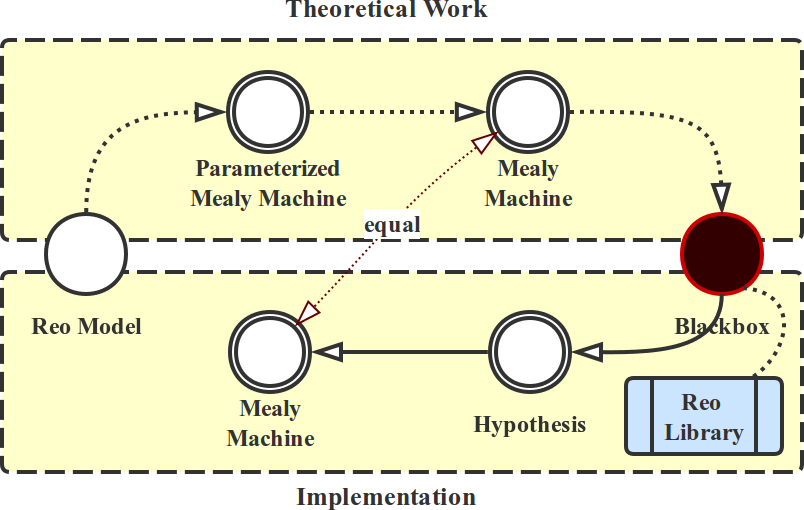
\includegraphics[width=.4\textwidth]{./images/howto.png}
  \end{center}
  \caption{The Active Learning Framework}
  \label{fig:howto}
\end{figure}

In this paper we address this question by proposing a active learning framework as shown in Figure
\ref{fig:howto} to automatically extract timed connector models from blackbox implementations. 
To achieve this goal, we first introduce \emph{parameterized Mealy machine} as a parameterized
semantics for timed Reo connectors, which can be transformed to concrete Mealy machines with a
given alphabet. Then the $L*$ algorithm \cite{DBLP:journals/iandc/Angluin87} is adapted and
optimized to extract Mealy machines with timed action from the connector implementations as
blackboxes. 

The rest of the paper is organized as follows: In Section
\ref{sec:preliminaries} we briefly illustrate some basic concepts, including the coordination
language Reo, Mealy machine, and active automata learning. Section \ref{sec:semantics} defines an
operational semantics of Reo, which is used in Section \ref{sec:activelearning} to show how to
extract Reo models from blackboxes by means of active learning. In Section
\ref{sec:experiment}, we discuss the implementation and optimization of the approach in
\texttt{Golang}. Finally, Section VI concludes the paper.

\section{Preliminaries} 
\label{sec:preliminaries}
\subsection{Reo Coordination Language} 
\label{sec:reo}
We provide here a brief overview of the main concepts in Reo. Further details can be found in
\cite{DBLP:journals/mscs/Arbab04, DBLP:journals/scp/BaierSAR06}.

Reo is a channel based exogenous coordination language proposed by F. Arbab in
\cite{DBLP:journals/mscs/Arbab04}. 
A coordinator in Reo, also called \emph{connector}, provides the protocol that controls and
organizes the communication, synchronization and cooperation among the components which
communicate through the connector. Connectors can be defined without dependence on components,
which makes Reo a powerful ``glue language'' in component-based
development\cite{DBLP:journals/sigsoft/Gill03}.

In Reo, complex connectors are made up of simpler ones. The atomic connectors are called
\emph{channels}, and each of them has two \emph{channel ends}. There are two types of channel ends:
\emph{source} and \emph{sink}. Source channel ends accept data into the channel, while sink
channel ends dispense data out of the channel. 

\begin{figure}[ht]
  \begin{center}
    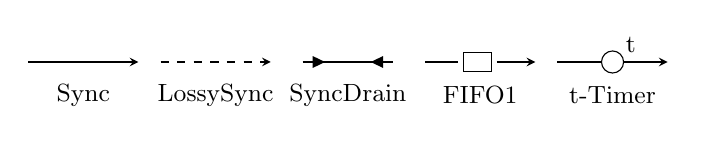
\begin{tikzpicture}[scale=1.4]

\tikzstyle{every node}=[font=\small]
\tikzstyle{label}=[draw=none]

\draw (0.5, -0.3) node[label] {Sync};
\draw (1.7, -0.3) node[label] {LossySync};
\draw (2.9, -0.3) node[label] {SyncDrain};
\draw (4.1, -0.3) node[label] {FIFO1};
\draw (5.3, -0.3) node[label] {t-Timer};

\sync{(0,0)}{(1,0)}{}
\lossysync{(1.2,0)}{(2.2,0)}{}
\syncdrain{(2.4,0)}{(3.4,0)}{}
\fifoe{(3.6,0)}{(4.6,0)}{}

\timer{(4.8,0)}{(5.8,0)}{node [above left] {t}}

\end{tikzpicture}

  \end{center}
  \caption{Basic Reo Channels}
  \label{fig:basic}
\end{figure}

Figure \ref{fig:basic} shows the graphical representation of some basic channel types in Reo, whose
behavior are described as follows:

\begin{itemize}
  \item [-] A \emph{Sync} channel accepts a data item from its source end iff the data item can be
    dispensed through its sink end simultaneously.
  \item [-] A \emph{LossySync} channel is always ready to accept data items. These items will be
    dispensed through its sink end simultaneously if possible, otherwise they will be lost.
  \item [-] A \emph{SyncDrain} channel has two source ends and no sink end. It can accept a data
    item through one of its source end iff a data item is also available to be accepted
    simultaneously through the other end. Then both items will be dropped.
  \item [-] A \emph{FIFO1} channel is an asychronous channel with a buffer cell. It accepts a
    data item whenever the buffer is empty. 
  \item [-] A t-timer channel accepts any data item from its source end, and later dispense it to
    its sink end after a delay of $t$ time units.
    \begin{footnote}
      Here the interpretation of t-Timer is a bit different as in other works like
      \cite{DBLP:conf/sefm/ArbabBBR04, DBLP:conf/tase/Meng12}, but we can easily transform between the
      two kinds of behavior by composing with some other basic channels.
    \end{footnote}
\end{itemize}

Channels are joint together in \emph{nodes}. There are three types of nodes:
\emph{source}, \emph{sink} and \emph{mixed} nodes, depending on whether all channel ends that
coincide on a node are source ends, sink ends or a combination of both.
(see in Figure \ref{fig:node})

\begin{figure}[ht]
  \begin{center}
    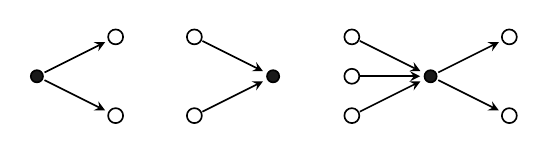
\begin{tikzpicture}[->,>=stealth',shorten >=1pt,auto,node distance=1.6cm,
  semithick]
  \tikzstyle{every node}=[font=\small]

  % source node
  \mixednode{(P-1)}{(-4,0)}{}
  \ionode{(P-2)}{(-3,0.5)}{}
  \ionode{(P-3)}{(-3,-0.5)}{}
  \sync{(P-1)}{(P-2)}{}
  \sync{(P-1)}{(P-3)}{}

  % sink node
  \mixednode{(S-1)}{(-1,0)}{}
  \ionode{(S-2)}{(-2,0.5)}{}
  \ionode{(S-3)}{(-2,-0.5)}{}
  \sync{(S-2)}{(S-1)}{}
  \sync{(S-3)}{(S-1)}{}

  % mixed node
  \ionode{(M-1)}{(0,0.5)}{}
  \ionode{(M-2)}{(0,0)}{}
  \ionode{(M-3)}{(0,-0.5)}{}
  \mixednode{(M-4)}{(1,0)}{}
  \ionode{(M-5)}{(2,0.5)}{}
  \ionode{(M-7)}{(2,-0.5)}{}
  \sync{(M-1)}{(M-4)}{}
  \sync{(M-2)}{(M-4)}{}
  \sync{(M-3)}{(M-4)}{}
  \sync{(M-4)}{(M-5)}{}
  \sync{(M-4)}{(M-7)}{}

\end{tikzpicture}

  \end{center}
  \caption{Source, Sink and Mixed Nodes in Reo}
  \label{fig:node}
\end{figure}

Components can be linked to source nodes or sink nodes. A component can write data items to its
corresponding source node only if the data item can be dispensed simultaneously to all source ends
on this node. Similarly, a component can read a data item only if there is at least one readable
sink end on its corresponding node. A mixed node non-determinstically selects and takes a data item
from one of its coincident sink ends and replicates it into all of its coincident source ends.

\begin{figure}[ht]
  \begin{center}
    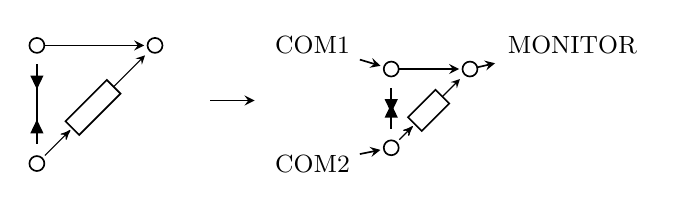
\begin{tikzpicture}[->,>=stealth',shorten >=1pt,auto,node distance=1.6cm,
  semithick]
  \tikzstyle{every node}=[font=\small]

  % draw the alternator
  \ionode{(P-A)}{(0,0)}{}
  \ionode{(P-B)}{(0,-1.5)}{}
  \ionode{(P-C)}{(1.5,0)}{}

  \sync{(P-A)}{(P-C)}{}
  \fifoe{(P-B)}{(P-C)}{}
  \syncdrain{(P-A)}{(P-B)}{}

  % draw the coordination
  \ionode{(C-A)}{(4.5,-0.3)}{}
  \ionode{(C-B)}{(4.5,-1.3)}{}
  \ionode{(C-C)}{(5.5,-0.3)}{}

  \sync{(C-A)}{(C-C)}{}
  \fifoe{(C-B)}{(C-C)}{}
  \syncdrain{(C-A)}{(C-B)}{}

  \node (COM1) at (3.5, 0) {COM1};
  \node (COM2) at (3.5, -1.5) {COM2};
  \node (MONI) at (6.8, 0) {MONITOR};
  \sync{(COM1)}{(C-A)}{}
  \sync{(COM2)}{(C-B)}{}
  \sync{(C-C)}{(MONI)}{}

  \sync{(2.2,-0.7)}{(2.8,-0.7)}{}

\end{tikzpicture}

  \end{center}
  \caption{Coordination with Reo Connectors}
  \label{fig:reoconnector}
\end{figure}

Figure \ref{fig:reoconnector} provides a simple example to illustrate how complex
connectors are constructed and used in coordination. In this example, we have three components
COM1,COM2 and MONITOR. With an \emph{alternator} connector as shown in Figure
\ref{fig:reoconnector}, MONITOR can obtain data items from COM1 and COM2 alternately. This example
has been implemented in \texttt{Golang} as shown in Section \ref{sec:reolib}.
Besides, all the connectors are supposed to have \emph{deterministic} behavior hereinafter to meet
the requirement of active learning algorithm L*.


\subsection{Mealy Machines} 

In this work, we use \emph{Mealy machines} to model Reo connectors.
Mealy machine was first proposed by George. H. Mealy in \cite{George1955A} as an extension of finite
state machine. Compared with other variants, Mealy machines are designed to model
reactive systems, where outputs of a machine are determined by not only its current state but also
the current inputs. Besides, Mealy machines are supposed to be \emph{input enabled}, which means
that all possible inputs should be acceptable in all states. In other words, if an input is invalid
for some state, we need to manually define an additional state to describe such exceptions.

Various forms of Mealy machines have been defined in the
literature\cite{George1955A,DBLP:journals/jcss/Broy14,DBLP:conf/sfm/SteffenHM11}. 
Since active automata learning requires the system-under-learn to be deterministic, in
this paper we take the deterministic Mealy machine model as defined in 
\cite{DBLP:conf/sfm/SteffenHM11}. 

\begin{definition}[Mealy machine]
  A Mealy machine is a 6-tuple $(S, s_0, I, O, \delta, \lambda)$ consisting of:
  \begin{itemize}
    \item[-] a finite set of states $S$
    \item[-] an initial state $s_0\in S$
    \item[-] a finite set of inputs $I$
    \item[-] a finite set of outputs $O$
    \item[-] an output function $\delta : S \times  I \rightarrow O$ mapping a pair
      of a state and an input to the corresponding output.
    \item[-] a transition function $\lambda : S \times I \rightarrow S$ mapping a pair of a
      state and an input to the corresponding successor state.
  \end{itemize}
\end{definition}

We say that a Mealy machine is \emph{finite} if the set $S$ of states and the set $I$ of inputs are
both finite. Hereinafter, Mealy machines are always supposed to be finite in this paper.


\subsection{Active Learning}
In this section, we briefly introduce the main ideas of active automata learning. 

Active learning \cite{settles2010active} is a special case of semi-supervised machine learning where
a learning algorithm is able to interactively query the target systems to obtain the desired outputs
under certain inputs. By well-designed query strategy, active learning is able to obtain more
accurate models with smaller dataset. 

\begin{figure}[ht]
  \begin{center}
    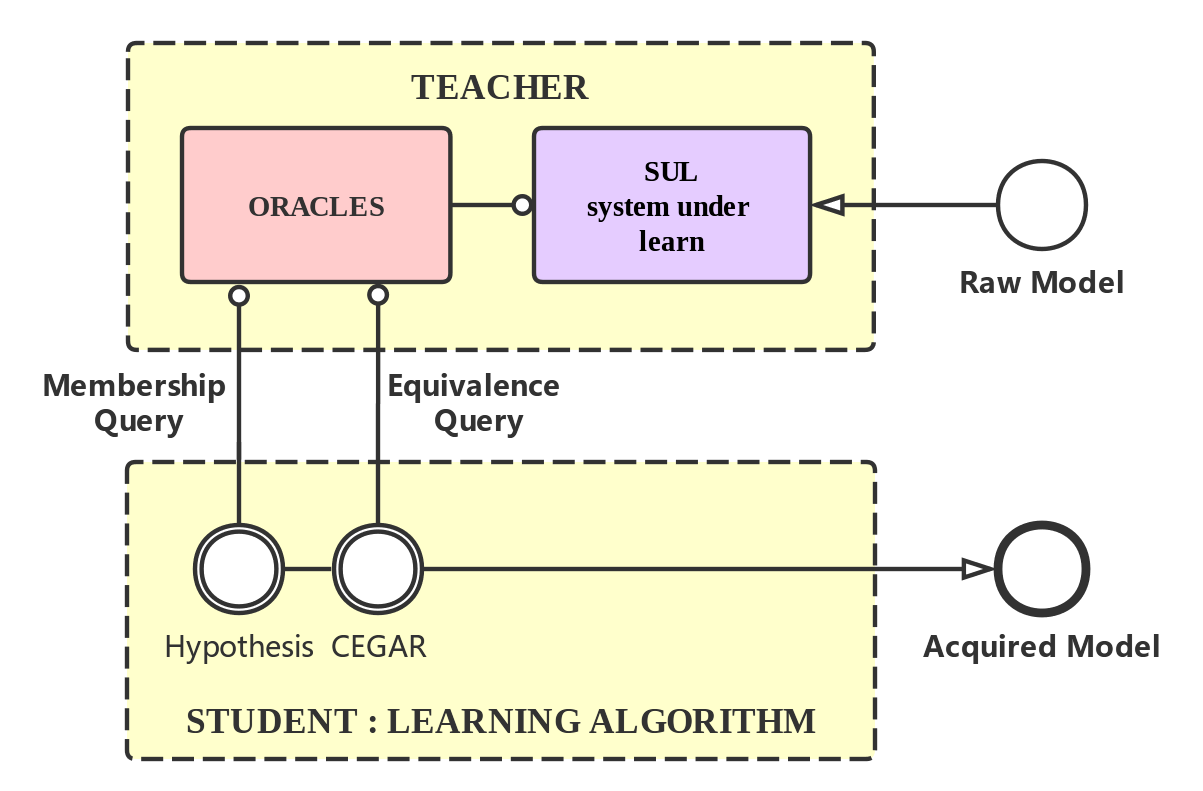
\includegraphics[width=.5\textwidth]{./images/activelearning.png}
  \end{center}
  \caption{Active Automata Learning}
  \label{fig:activelearning}
\end{figure}

Figure \ref{fig:activelearning} shows the sketch of active learning, wherein:
\begin{itemize}
  \item[-] \emph{Teacher} and \emph{Student}: Active learning is an interactive process where
    students ask questions and teachers answer. Here learning algorithm plays the role of student.
  \item[-] \emph{Oracles} is an interface specifying which kind of questions can be answered by the
    teacher.
  \item[-] \emph{SUL} is an abbreviation of System Under Learn. In this paper, we take blackbox
    models as our SULs.
  \item[-] \emph{CEGAR} indicates Counter-Example Guided Abstraction
    Refinement\cite{DBLP:conf/cav/ClarkeGJLV00}. In active learning, we need counter-examples to
    guide us on further queries and cover the undistinguished states.
\end{itemize}

When applying active automata learning on some model, we assume that the model should be equivalent
to some \emph{Mealy machine}, i.e., a deterministic model accepting a finite set of inputs and
mapping them to a finite set of outputs.

Such a model is encapsulated as a \emph{teacher} by the \emph{Oracle}, which handles
all communication with the model. The oracle also serves as a so-called \emph{Minimal Adequate Teacher}
interface, which is responsible for two types of queries. 

\begin{itemize}
  \item[-] \textbf{Membership Query} (hereinafter referred to as \emph{mq}) In grammar-learning
    \cite{DBLP:journals/iandc/Angluin87}, \emph{mq} checks if a word is a member of certain language
    defined by the given grammar. When it comes to
    automata learning, \emph{mq} is supposed to provide \emph{simulation results} for given input
    sequences.
  \item[-] \textbf{Equivalence Query} (hereinafter referred to as \emph{eq}) Given a hypothesis
    (usually constructed by the learning algorithm), \emph{eq} checks whether the hypothesis is
    equivalent to the system-under-learn and generates a counter-example if needed. Generally, 
    \emph{eq} is irrealizable when SUL is a blackbox. So we tactically use $mq$ to achieve the
    approximate results.
\end{itemize}

These queries are given by \emph{learning algorithms}, or so-called \emph{students} in Figure
\ref{fig:activelearning}. From the \emph{mq} results, a learning algorithm constructs a
\emph{hypothesis} and then check it with \emph{eq}. If counter-examples are found, we turn back and
repeat the hypothesis construction until the equivalence query returns \emph{true}.

More details on the active automata learning algorithm will be presented in Section
\ref{sec:activelearning}. 


\section{Timed Connectors as Mealy Machines}
\label{sec:semantics}

In this section, we illustrate how to transform a timed connector into a Mealy machine with timed
action.
Since time is not involved in original Mealy machine, we first discuss how to formalize the time
dimension in Mealy machine. After that, we present the notion of \emph{parameterized Mealy
machine} as a bridge between connectors and Mealy machines.

\subsection{Time Domain}
Time has been investigated in several extensions of Reo. For example, timed
Reo\cite{DBLP:conf/sefm/ArbabBBR04, DBLP:conf/fmoods/MengA07}, hybrid Reo\cite{DBLP:conf/icfem/ChenSS14}, etc.
Generally, these models are designed to handle real-time behavior where time is defined on the
real number field $\mathbb{R}$. However, there are also some works like
\cite{DBLP:journals/fmsd/PrabhakarDM015} where
rational time indeed  makes things easier. In this paper, we choose the rational number field
$\mathbb{Q}$ as our time domain, which simplifies discretization of timed behavior greatly.

As presented in section \ref{sec:reo}, all real-time behavior in timed Reo comes with a finite set
of timed channels. We use
$t_i\in\mathbb{Q}, i=1,2,\dots,n$ to denote the delays of these timed channels, and then we can define a precision
function $prec$ which calculate a gcd-style \emph{maximal time precision}:
\[
prec(t_1,\dots,t_n) = \max\{T\in\mathbb{Q}|\forall t_i.\exists n_i\in\mathbb{N}.t_i=n_i\cdot T\}
\]
It's easy to prove that such a $T$ always exists.

In embedded systems, the maximal time precision is also called ``clock-period'', which is the basic
time unit provided by an oscillator. For example, a widely-used Intel-80C51 microcontroller works
under the frequency 16Mhz, where the clock-period is $62.5$ns. A reasonable assumption comes that
such a maximal time precision $dt=prec(t_1,\dots,t_n)$ should always be provided to make sure
different components are able to work together. Then all $t_i$-Timers can be seen as $n_idt$-Timers
for some $n_i$ and we use $n_i$-Timers instead in the following sections.

Besides, we're going to add a ``T'' action in Mealy machines. It indicates that the corresponding
transition will take one time unit to finish.

\subsection{Parameterized Mealy Machine}
We present a model named \emph{parameterized Mealy machine} to model timed connectors. PMM is
supposed to behave as a bridge between Mealy machines and timed connectors. Connectors are firstly
defined as PMMs, and composed by \emph{product} and \emph{link} operators. Then, concrete
Mealy-machine model can be generated from the PMM model.
Following the formal definition of Mealy machine in Section \ref{sec:preliminaries}, we define the
\emph{parameterized Mealy machine} as follows. 

\begin{definition}[Parameterized Mealy Machine]
  A \emph{Parameterized Mealy Machine} with a parameter $\Sigma$ is defined as a 6-tuple
  $\mathcal{PM}=\langle S, s_0, I, O, \delta, \lambda\rangle$ where 
  \begin{itemize}
    \item[-] The value of $\Sigma$ is a \emph{finite} data set (hereinafter referred as
      alphabet), e.g. $\{a,b\}$
    \item[-] $S$ maps an alphabet to a \emph{finite} set of states.
    \item[-] $s_0$ is the initial state. It satisfies $\forall \Sigma.s_0\in S(\Sigma)$
    \item[-] $I$ is a finite set of source-ends.
    \item[-] $O$ is a finite set of sink-ends.
    \item[-] $\delta$ maps an alphabet to an \emph{output function}. We use
      $\delta(\Sigma):S(\Sigma)\times Input(\Sigma,I,O)\rightarrow Output(\Sigma,O)$ to denote the
      output function.
    \item[-] $\lambda$ maps an alphabet to a \emph{transition function}. We use
      $\lambda(\Sigma):S(\Sigma)\times Input(\Sigma,I,O)\rightarrow S(\Sigma)$ to denote the
      transition function.
  \end{itemize}
\end{definition}

In the definition above, \emph{Input} and \emph{Output} are used to generate the set of input actions
and output actions from the corresponding alphabets and source/sink ends. $Input(\Sigma,I,O)$ is
defined as a set of functions on $I\cup O$ and an additional \emph{time action} T,  
where for all $f\in Input(\Sigma,I,O)\backslash \{T\}$ we have
\[
\forall i\in I.f(i)\in \Sigma\cup\{\bot\}\land \forall o\in O.f(o)\in\{\rread, \rnoread\}
\]
where we use $\bot$ to indicate that there is \emph{no} data item on a channel end. 
Besides, $\rread$ means that a sink end is ready for writing, $\rnoread$ otherwise. 
In the same way,
$Output(\Sigma,O)$ is defined as a set of functions on $O$, with an additional symbol
$\rblock$ indicating an input failure. Similarly, for all $f\in
Output(\Sigma,O)\backslash\{\rblock\}$,
\[
\forall o\in O. f(o)\in \Sigma\cup\{\bot\}
\]

\begin{example}[Input and Output]
  If we have a simple alphabet with only one item $d_0$, a source-end named $A$, and a
  sink-end named $B$, the input actions would be
  \begin{eqnarray*}
    & & Input(\{d_0\},\{A\},\{B\}) \\
    & = & \{\{A\mapsto d_0,B\mapsto\rread\},\{A\mapsto d_0,B\mapsto\rnoread\}, \\
    & & \{A\mapsto\bot,B\mapsto\rread\}, \{A\mapsto\bot,B\mapsto\rnoread\},T\}
  \end{eqnarray*}
  and its output actions
  \[
  Output(\{d_0\},\{A\},\{B\}) =\{\{B\mapsto d_0\},\{B\mapsto \bot\}, \rblock\}
  \]
\end{example}

We use $\varnothing$ to denote the empty output when no data item is written to any sink end.
For example, in this case $\{B\mapsto\bot\}$ can be briefly denoted as $\rempty$.

Parameterized Mealy machines can be seen as an abstraction of Mealy machines, and we
still need a convert function between the two models.

\begin{definition}[Concretize Mapping]
  We use $\smap{\mathcal{PM}}_{\Sigma}$ to denote the concrete Mealy machine which is determined by
  an abstract parameterized Mealy machine $\mathcal{PM}$ and the alphabet $\Sigma$. Apparently
  $\smap{\mathcal{PM}}_{\Sigma}$ can be described as
  \begin{eqnarray*}
    \smap{\mathcal{PM}}_{\Sigma} &=& 
    \langle
    \mathcal{PM}.S(\Sigma), \mathcal{PM}.s_0, \\
    & & Input(\Sigma, \mathcal{PM}.I, \mathcal{PM}.O), Output(\Sigma, \mathcal{PM}.O), \\
    & & \mathcal{PM}.\delta(\Sigma), \mathcal{PM}.\lambda(\Sigma),
    \rangle
  \end{eqnarray*}
\end{definition}

Now we can use PMMs to specify timed Reo. Here we take the asynchronous channel (FIFO1), the
synchronous channel (Sync) and the timed channel (Timer) as examples. For simplicity, we use $A=\_$
to indicate that there is no constraint on channel end $A$.

\begin{example}[FIFO1]
  \label{example:pmmfifo}
  The PMM of a FIFO1 with source end $A$ and sink end $B$ can be defined as follows.
  \begin{itemize}
    \item[-] $S(\Sigma)=\{q_0\}\cup\{q_d|d\in\Sigma\}$
    \item[-] $I=\{A\}$, $O=\{B\}$, $s_0=q_0$
    \item[-] output function
      \begin{small}
        \begin{displaymath}
          \delta(\Sigma)(s,i)=\left\{
          \begin{array}[ht]{ll}
            \rempty & s=q_0\land i=\{A\mapsto\_,B\mapsto\rnoread\} \\
            \rblock & s=q_0\land i=\{A\mapsto d',B\mapsto\rread\} \\
            \rblock & s=q_0\land i=\{A\mapsto\bot,B\mapsto\rread\} \\
            \rempty & s=q_d\land i=\{A\mapsto\bot,B\mapsto\rnoread\} \\     
            \{B\mapsto d\} & s=q_d\land i=\{A\mapsto\_,B\mapsto\rread\}\\
            \rblock & s=q_d\land i=\{A\mapsto d',B\mapsto \rnoread\} \\
          \end{array}
          \right.
        \end{displaymath}
      \end{small}
    \item[-] transition function
      \begin{small}
        \begin{displaymath}
          \lambda(\Sigma)(s,i)=\left\{
          \begin{array}[ht]{ll}
            q_{d'} & s=q_0\land i=\{A\mapsto d',B\mapsto\_\} \\
            q_{d'} & s=q_{d}\land i=\{A\mapsto d',B\mapsto \rread\} \\
            q_{d} & s=q_{d}\land i=\{A\mapsto \_,B\mapsto \rnoread\} \\
            q_0 & otherwise \\
          \end{array}
          \right.
        \end{displaymath}
      \end{small}
  \end{itemize}
\end{example}

Besides, the concrete Mealy machine (where $\Sigma=\{d\}$) is shown in Figure \ref{fig:pmmfifo},
where labels of edges are in form of $\frac{input}{output}$. All $\rblock$ edges are ignored for
clearance.
\begin{figure}[ht]
  \begin{center}
    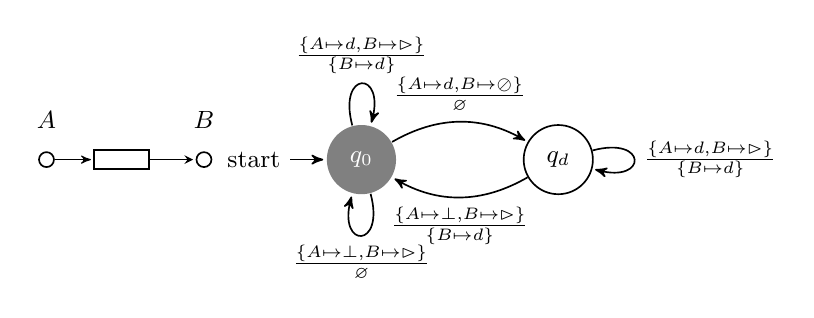
\begin{tikzpicture}[->,>=stealth',shorten >=1pt,auto,node distance=1.6cm,
  semithick]
  \tikzstyle{every node}=[font=\small]
  \ionode{(P-A)}{(-4,0)}{(-4,0.5) node {$A$}}
  \ionode{(P-B)}{(-2,0)}{(-2, 0.5) node {$B$}}
  
  \fifoe{(P-A)}{(P-B)}{}

  \tikzstyle{every state}=[fill=white,text=black,font=\small]
  \tikzstyle{init}=[fill=gray,draw=none,text=white]

  \node[initial,state,init] (Q0)                     {$q_{0}$};
  \node[state]         (QA)  [right = of Q0]    {$q_{d}$};

  \path
  (Q0)
  edge  [bend left]     node {$\frac{\{A\mapsto d, B\mapsto \rnoread\}}{\varnothing}$} (QA)
  edge  [loop below]    node {$\frac{\{A\mapsto \bot, B\mapsto \rread\}}{\varnothing}$} (QA)
  edge  [loop above]    node {$\frac{\{A\mapsto d, B\mapsto \rread\}}{\{B\mapsto d\}}$} (QA)
  (QA)
  edge  [bend left]     node {$\frac{\{A\mapsto \bot,B\mapsto \rread\}}{\{B\mapsto d\}}$} (Q0)
  edge  [loop right]    node {$\frac{\{A\mapsto d,B\mapsto \rread\}}{\{B\mapsto d\}}$} (QA)
  ;
\end{tikzpicture}


  \end{center}
  \caption{PMM-based Semantics of $\smap{FIFO1}_\Sigma$, where $\Sigma=\{d\}$}
  \label{fig:pmmfifo}
\end{figure}

\begin{example}[Sync]
  The PMM of a Sync with a source-end A and a sink-end B can be defined as:
  \begin{itemize}
    \item[-] $S(\Sigma)=\{q_0\}$, $I=\{A\}$, $O=\{B\}$, $s_0=q_0$
    \item[-] output function
      \begin{displaymath}
        \delta(\Sigma)(s,i)=\left\{
        \begin{array}[ht]{ll}
          \rempty & i=\{A\mapsto\bot,B\mapsto\rnoread\} \\
          \{B\mapsto d\} & i=\{A\mapsto d,B\mapsto\rread\}\\
          \rblock & i=\{A\mapsto\bot,B\mapsto\rread\} \\
          \rblock & i=\{A\mapsto d,B\mapsto\rnoread\} \\
        \end{array}
        \right.
      \end{displaymath}
    \item[-] transition function $\lambda(\Sigma)(s,i)=q_0$.
  \end{itemize}
\end{example}

\begin{example}[n-Timer]
  The PMM of an n-Timer with a source-end A and a sink-end B can be defined as:
  \begin{itemize}
    \item[-] $S(\Sigma)=\{q_{i,d}|0\leq i\leq n, d\in \Sigma\}\cup\{q_0\}$
    \item[-] $I=\{A\}$, $O=\{B\}$, $s_0=q_0$
    \item[-] output function
      \begin{small}
        \begin{displaymath}
          \delta(\Sigma)(s,i)=\left\{
          \begin{array}[ht]{ll}
            \{B\mapsto d\} & s=q_{n,d}\land i=\{A\mapsto \_,B\mapsto \rread\}\\
            \rblock & s=q_{n,d}\land \\
            & (i=T\lor i=\{A\mapsto \_,B\mapsto \rnoread\}) \\
            \rblock & s=q_{j,d}\land 0 \leq j < n\land \\
            & (i=\{A\mapsto \_,B\mapsto \rread\}\lor \\
            & i=\{A\mapsto d,B\mapsto \_\})\\
            \rempty & otherwise\\
          \end{array}
          \right.
        \end{displaymath} 
      \end{small}
    \item[-] transition function
      \begin{small}
        \begin{displaymath}
          \lambda(\Sigma)(s,i)=\left\{
          \begin{array}[ht]{ll}
            q_{0,d} & s=q_0 \land i=\{A\mapsto d,B\mapsto \_\} \\
            q_{j+1,d} & s=q_{j,d}\land i=T\land0 \leq j < n\\
            q_0 & s=q_{n,d}\land i=\{A\mapsto \bot,B\mapsto \rread\} \\
            q_{0,d'} & s=q_{n,d}\land i=\{A\mapsto d',B\mapsto \rread\} \\
            q_0 & s=q_{n,d} \land i=T \\
            s & otherwise \\
          \end{array}
          \right.
        \end{displaymath}
      \end{small}
  \end{itemize}
\end{example}

Similarly, we can use PMMs to describe the behavior of other basic timed Reo
channels. Now we show how to compose these channels into more complicated connectors.

\begin{definition}[Product]
  The product operator \emph{prod} of two PMMs
  \[
  \mathcal{PM'} = prod(\mathcal{PM}_1,\mathcal{PM}_2)\mbox{ if }\mathcal{PM}_2.O\cap
  \mathcal{PM}_1.I=\varnothing
  \]
  is defined as follows.
  \begin{itemize}
  	\item[-] $\forall\Sigma. \mathcal{PM}'.S(\Sigma)=\mathcal{PM}_1.S(\Sigma)\times \mathcal{PM}_2.S(\Sigma)$
    \item[-] $\mathcal{PM}'.I=(\mathcal{PM}_1.I\cup \mathcal{PM}_2.I)\backslash \mathcal{PM}_1.O$
    \item[-] $\mathcal{PM}'.O=(\mathcal{PM}_1.O\cup \mathcal{PM}_2.O)\backslash \mathcal{PM}_2.I$
  \end{itemize}
  \emph{(Here we assume that sink ends of $\mathcal{PM}_1$ can be connected to source ends $\mathcal{PM}_2$, but not
  vise versa)}
  \begin{itemize}
    \item[-] $\mathcal{PM}'.s_0=(\mathcal{PM}_1.s_0, \mathcal{PM}_2.s_0)$
    \item[-] $\forall\Sigma. \mathcal{PM}'.\delta(\Sigma)((s_1,s_2), i)=$
      \begin{displaymath}
        \left\{
        \begin{array}[ht]{ll}
          (Out_1 \cup Out_2)\downarrow_{\mathcal{PM}'.O} & Out_1\neq\rblock\land Out_2\neq\rblock \\
          \rempty & i = T \\
          \rblock & otherwise \\
        \end{array}
        \right.
      \end{displaymath}
      where we have
      \begin{itemize}
        \item[*] $In_1 = i\downarrow_{\mathcal{PM}_1.I}$
        \item[*] $Out_1 = \mathcal{PM}_1.\delta(\Sigma)(s_1,In_1)$
        \item[*] $In_2 = (Out_1 \cup i)\downarrow_{\mathcal{PM}_2.I}$
        \item[*] $Out_2 = \mathcal{PM}_2.\delta(\Sigma)(s_2,In_2)$
      \end{itemize}
    \item[-] $\forall\Sigma. \mathcal{PM}'. \lambda(\Sigma)((s_1,s_2),i)=(s_1',s_2')$
      where we have
      \begin{itemize}
        \item[*] $s_1' = \mathcal{PM}_1.\lambda(\Sigma)(s_1,In_1)$
        \item[*] $s_2' = \mathcal{PM}_2.\lambda(\Sigma)(s_2,In_2)$
      \end{itemize}
  \end{itemize}
\end{definition}

The idea in \emph{production} is quite simple. The output of $\mathcal{PM}_1$ would be provided as part of the
input of $\mathcal{PM}_2$. Time actions T is only executed simultaneously between $\mathcal{PM}_1$ and $\mathcal{PM}_2$.

As mentioned in the notation above, we cannot connect a sink end of $\mathcal{PM}_2$ to a source end of
$\mathcal{PM}_1$, which makes it difficult to construct connectors like alternator in Figure
\ref{fig:reoconnector}. To address the problem, we define a \emph{link} operation to connect sink
ends and source ends in the same connector.

\begin{definition}[Link]
  The \emph{link} operator constructs connector by connecting a sink end $\OUT$ to a source end $\IN$
  within the same connector.   
  \[
  \mathcal{PM}' = link(\mathcal{PM}, \OUT, \IN)
  \]
  Here we assume that $\IN\in \mathcal{PM}.I$ and $\OUT\in \mathcal{PM}.O$.

  \begin{itemize}
  	\item[-] $\forall\Sigma. \mathcal{PM}'.S(\Sigma)=\mathcal{PM}.S(\Sigma)$
    \item[-] $\mathcal{PM}'.I=\mathcal{PM}.I\backslash\{\IN\}$
    \item[-] $\mathcal{PM}'.O=\mathcal{PM}.O\backslash\{\OUT\}$
    \item[-] $\mathcal{PM}'.s_0=\mathcal{PM}.s_0$
    \item[-] $\forall\Sigma, i\in
      Input(\Sigma,\mathcal{PM}'.I,\mathcal{PM}'.O).\mathcal{PM}'.\delta(\Sigma)(s,i)=$
      \begin{small}
        \begin{displaymath}
          \left\{
          \begin{array}[h]{lr}
            \rempty & i=T \\
            \mathcal{PM}.\delta(\Sigma)(s,i\cup\{\IN:d\})\downarrow_{\mathcal{PM}'.O} & (*)\\
            \rblock & otherwise \\
          \end{array}
          \right.
        \end{displaymath}
      \end{small}
      where the condition (*) is defined as
      \[
      \exists d.\mathcal{PM}.\delta(\Sigma)(s,i\cup\{\IN:d\})(\OUT)=d
      \]
    \item[-] $\forall\Sigma, i\in
      Input(\Sigma,\mathcal{PM}'.I,\mathcal{PM}'.O).$
      \begin{small}
        \begin{displaymath}
          \mathcal{PM}.\lambda(\Sigma)(s,i)=
          \left\{
          \begin{array}[ht]{lr}
            \mathcal{PM}.\lambda(\Sigma,T) & i=T \\
            \mathcal{PM}.\lambda(\Sigma,i\cup\{\IN:d\}) & (*)\\
            s & otherwise \\
          \end{array}
          \right.
        \end{displaymath}
      \end{small}
  \end{itemize}
\end{definition}

With \emph{link} and \emph{prop} defined, connectors can be constructed by simpler ones in
form of PMMs. It will be transformed into a concrete Mealy machine later, once the alphabet $\Sigma$
is provided.

\section{From Blackbox to Timed Connectors} 
\label{sec:activelearning}
In this section, we use L* algorithm to extract Reo coordinators from blackbox
implementations in 3 steps:
\emph{constructing hypothesis}, \emph{enclosing hypothesis} and \emph{validating hypothesis}. Besides,
here the input and output symbols of the blackbox are provided as $\mathcal{I}$ and $\mathcal{O}$,
and the blackbox implementation is supposed to be equivalent to a Mealy machine where all states are
reachable.

\subsection{Observation Table}
\emph{Observation Tables}, proposed in \cite{DBLP:journals/iandc/Angluin87}, are used to construct
hypothetical Mealy machines from the results of membership queries.

Mealy machines are composed of \emph{states} and \emph{transitions}.
As for blackboxes, input sequence $s\in\mathcal{I}^*$ can be used to denote its state 
after executing $s$. Similarly, for all $a\in\mathcal{I}$, we use $sa$ to denote the successor
state of $s$ after executing $a$.
However, under such notations, there are \emph{infinite} number of states, among which most are
reduplicate.

States are distinguished, usually, by their \emph{subsequent behavior}. Suppose $s_1\neq s_2\in
\mathcal{I}^*$, we say the corresponding of states $s_1$ and $s_2$ are equivalent iff $\forall d\in
\mathcal{I}^+. mq(s_1d)=mq(s_2d)$. Since we can never check it on every $d\in\mathcal{I}^+$, an
alternative way is to use a set of \emph{suffixes} to distinguish them approximately.
\begin{definition}[$D$-Equivalence]
  provided with a set of suffixes $D\subset\mathcal{I}^+$, we say the corresponding states of
  $s_1,s_2\in\mathcal{I}^*$ are $D$-equivalent (denoted as $s_1\sim_D s_2$)
  iff $mq(s_1d) = mq(s_2d)$ for all $d\in D$.
\end{definition}

Now we use \emph{access sequence} to describe the states. Given an input sequence $s$, the access
sequence of $s$ is defined as
\[
acc(s,D)=\min\{s'\in\mathcal{I}^*|s'\sim_D s\}
\]

Formally, an observation table (see in Figure \ref{fig:hypo}) is determined by a tuple $(S,D)$ where
$S\subset\mathcal{I}^*$ is a set of the access sequences of states and $D\subset\mathcal{I}^*$
is a set of suffixes. In such tables, columns are labelled with suffixes in $D$, and rows are
labelled with input sequences. As shown in the example, rows are divided into two parts. The upper
part, labelled with access sequence $s\in S$, denotes the states covered in the current hypothesis.
The lower part, labelled with sequences in $\{sa|s\in S,a\in\mathcal{I}\}\backslash S$ (representing
any potentially unclosed transition) denotes all the transitions outside $s\in S$. A cell with row
label $s$ and column label $d$ is filled with $mq(sd)$.

An observation table $(S,D)$ is \emph{closed} if 
\[
\forall s\in S,a\in\mathcal{I}.\exists s'\in S. sa\sim_D s'
\]

From a closed observation we can construct a hypothetical Mealy machine in a straight-forward way.
The Mealy machine $\mathcal{H}=\langle S,s_0,\mathcal{I},\mathcal{O},\delta,\lambda\rangle$ is
constructed from $obs$ as follows:
\begin{itemize}
  \item[-] Every state in $S$ corresponds to an input sequence in $obs.S$
  \item[-] $s_0$ corresponds to the empty sequence $\varepsilon$
    
    \emph{(we use input sequences to indicate their corresponding states in following parts)}
  \item[-] $\delta(s,a)=mq(sa)$
  \item[-] $\lambda(s,a)=acc(sa,obs.D)$. Since $obs$ is closed, we always have $\lambda(s,a)\in S$.
\end{itemize}

Algorithm \ref{alg:buildtable} shows how to build an closed observation table.

\begin{algorithm} 
  \caption{CloseTable} 
  \label{alg:buildtable}
  \small
  \KwIn{An oracle interface $mq$, An input actions $\mathcal{I}$, An observation table $obs$}
  \KwOut{A closed observation table $obs$} 
  \Repeat{$unclosed=\varnothing$}
  {
    $next=\{st|\forall s\in obs.S,\forall t\in \mathcal{I}\}\backslash obs.S$\;
    $unclosed=\{seq\in next|\forall a\in obs.S, seq \not\sim_{obs.D} a\}$\;
    $obs.S$ = $obs.S\cup unclosed$\;
  }
  \Return $obs$\; 
\end{algorithm}

Taking a 2-Timer channel as an example, we now illustrate how this algorithm works. 
We assume that the source end of this 2-Timer channel is $A$, the sink end is $B$, and the alphabet
is $\{a\}$. We briefly denote $\{A:a,B:\rnoread\}$ and other input/output actions in form of
$a,\rnoread$.

Firstly, $obs.S$ is initialized with the initial state (denoted by $\varepsilon$), and $obs.D$ is
initialized with all one-step suffixes.
Then we will explore all the access sequences in $obs.S$ and calculate its successors. Here the
$unclosed$ set consists of access sequences that has no equivalent fellow in $obs.S$. 
For example, figure \ref{fig:hypo} shows the $obs$ of a 2-Timer channel after the first
iteration. The five successors of $\varepsilon$ is presented as the bottom part of the table, where
four are equivalent with $\varepsilon$ but $a,\rnoread$ is not. Therefore, we take $a,\rnoread$ as a
brand-new state and all of its successors need further exploration (see in the hypothesis Mealy
machine presented in the following figure).

\begin{figure}[ht]
  \begin{center}
    \begin{displaymath}
      \begin{array}{l||ccccc||c}
        \hline
        & a,\rread & \bot,\rread & a,\rnoread & \bot,\rnoread & T & \mbox{AccessSequence}\\
        \hline\hline
        \varepsilon & \rblock & \rblock & \rempty & \rempty & \rempty & \varepsilon\\
        \hline
        a,\rread & \rblock & \rblock & \rempty & \rempty & \rempty & \varepsilon\\
        \bot,\rread & \rblock & \rblock & \rempty & \rempty & \rempty & \varepsilon \\
        \rowcolor[gray]{.9}
        a,\rnoread & \rblock & \rblock & \rblock & \rempty & \rempty & \mbox{NO MATCH}\\
        \bot,\rnoread & \rblock & \rblock & \rempty & \rempty & \rempty & \varepsilon \\
        T & \rblock & \rblock & \rempty & \rempty & \rempty \varepsilon & \varepsilon \\
        \hline
      \end{array}
    \end{displaymath}
    % 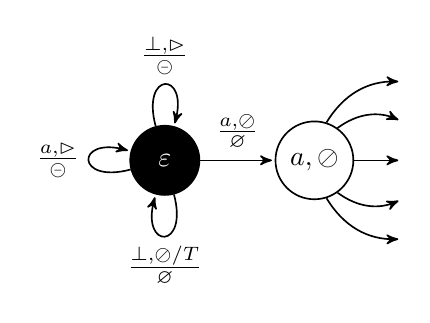
\begin{tikzpicture}[->,>=stealth',shorten >=1pt,auto,node distance=1.9cm,
  semithick]
  \tikzstyle{initial}=[fill=black, text=white]

  \node[initial,state] (Q0)               {$\varepsilon$};
  \node[state]         (Q1) [right of=Q0] {$a,\rnoread$};
  
  \path
  (Q0) edge [loop left]  node {$\frac{a,\rread}{\rblock}$} (Q0)
  (Q0) edge [loop above] node {$\frac{\bot,\rread}{\rblock}$} (Q0)
  (Q0) edge              node {$\frac{a,\rnoread}{\rempty}$} (Q1)
  (Q0) edge [loop below] node {$\frac{\bot,\rnoread/T}{\rempty}$} (Q0)
  (Q1) edge [bend left]  node {} (3,1)
  (Q1) edge [bend left]  node {} (3,0.5)
  (Q1) edge              node {} (3,0)
  (Q1) edge [bend right] node {} (3,-0.5)
  (Q1) edge [bend right] node {} (3,-1)
  ;
\end{tikzpicture}


  \end{center}
  \caption{Observation Table and Corresponding Hypothesis}
  \label{fig:hypo}
\end{figure}

In the second iteration, we explore the successors of $a,\rnoread$. Fortunately, now every
successor has a equivalence fellow in $obs.S$ (\emph{itself}). Consequently, the algorithm terminates
with a closed hypothesis where all the unclosed edge shown in Figure \ref{fig:hypo} turn into
self-loop.

\begin{figure}[ht]
  \begin{center}
    \begin{small}
      \begin{displaymath}
        \begin{array}{l||ccccc||c}
          \hline
          & a,\rread & \bot,\rread & a,\rnoread & \bot,\rnoread & T & \mbox{AccessSequence}\\
          \hline\hline
          \varepsilon & \rblock & \rblock & \rempty & \rempty & \rempty & \varepsilon \\
          \hline
          a,\rread & \rblock & \rblock & \rempty & \rempty & \rempty & \varepsilon\\
          \bot,\rread & \rblock & \rblock & \rempty & \rempty & \rempty & \varepsilon \\
          a,\rnoread & \rblock & \rblock & \rblock & \rempty & \rempty & a,\rnoread \\
          \bot,\rnoread & \rblock & \rblock & \rempty & \rempty & \rempty & \varepsilon \\
          T & \rblock & \rblock & \rempty & \rempty & \rempty & \varepsilon \\
          \hline
          a,\rnoread-a,\rread & \rblock & \rblock & \rblock & \rempty & \rempty & a,\rnoread \\
          a,\rnoread-\bot,\rread & \rblock & \rblock & \rblock & \rempty & \rempty & a,\rnoread \\
          a,\rnoread-a,\rnoread & \rblock & \rblock & \rblock & \rempty & \rempty & a,\rnoread \\
          a,\rnoread-\bot,\rnoread & \rblock & \rblock & \rblock & \rempty & \rempty & a,\rnoread \\
          a,\rnoread-T & \rblock & \rblock & \rblock & \rempty & \rempty & a,\rnoread \\
          \hline
        \end{array}
      \end{displaymath}
    \end{small}
  \end{center}
  \caption{A Closed Observation Table}
  \label{fig:hypo2}
\end{figure}

\subsection{Counter Examples' Analysis} 
Apparently, the closed hypothesis presented in Figure \ref{fig:hypo2} is different with the 2-Timer
channel. It's easy to find a counter-example $s_0=a,\rnoread-T-T-\bot,\rread$ where $mq(s)=a$ while
according to the hypothesis, the result should be $\rempty$. In this section, we show how to
find and analyze counter-examples using the method in \cite{DBLP:conf/sfm/SteffenHM11}. 

Firstly, we give a formal definition of \emph{counter examples}. With a observation table $obs$ and
a sequence $s$, we use $hq(obs,s)$ to denote the execution result of its corresponding hypothesis
$\mathcal{H}$ under the input sequence
$s$. Obviously we have $hq(obs,s) = mq(acc(s')a)$ where $s=s'a,a\in\mathcal{I}$.

\begin{definition}[Counter Example]
  an input sequence $s$ is a counter example of $obs$ iff $mq(s)\neq hq(obs,s)$.
\end{definition}

Now we consider the reason that lead to existance of counter examples. Since
the suffix set $D$ is used to distinguish states, the existance of counter-examples
shows that the current suffix set $D$ is not powerful enough to recognize the uncovered states in
$next$ (see in Algorithm \ref{alg:buildtable}).

Considering a counter example $s$, we need a new suffix to distinguish the uncovered states, which
can be calculated by Suffix($s,obs$):
\[
\max\{d\in\mathcal{I}^+|s=s'd, mq(acc(s',obs.D)d)\neq mq(s)\}
\]
After appending $d$ in $D$, we can prove that at least one new state will be found.

\begin{theorem}
\end{theorem}

The whole L* algorithm can be concluded as follows.
\begin{algorithm} 
  \caption{L*} 
  \label{alg:lstar}
  \KwIn{Oracle interface $mq,eq$, Input actions $\mathcal{I}$}
  \KwOut{Observation table $obs$} 
  $obs.S$ initialized as empty\;
  $obs.D$ initialized as $\{\{i\}|i\in\mathcal{I}\}$\;
  \Repeat{$ce=true$}{
    $obs$ = CloseTable($mq$, $\mathcal{I}$, $obs$)\;
    $ce=eq(obs)$\;
    \If {$ce\neq true$} {
      D.append(Suffix(s))\;
    }
  }
  \Return $obs$\; 
\end{algorithm}




\section{Experiments} 
\label{sec:experiment}

Both \emph{Reo Coordination Models} and \emph{Adapted L* Algorithm} are implemented in
Golang\cite{golang}, which is widely known for its elegant design and impressive efficiency.
Moreover, with a CSP-style\cite{DBLP:books/ph/Hoare85} cocurrency model,\texttt{Golang} shares many
similar ideas with Reo, and in turn makes our implementation much more natural.

All the following experiments are coded under Golang \emph{1.2.1} and executed on a laptop with 8GB
of RAM and a Core i7-3630 CPU. The source code is available at
\url{https://github.com/liyi-david/reo-learn}.

\subsection{Case Study}
A simple example of timed connector is presented to show how L* works.
\begin{figure}[ht]
  \begin{center}
    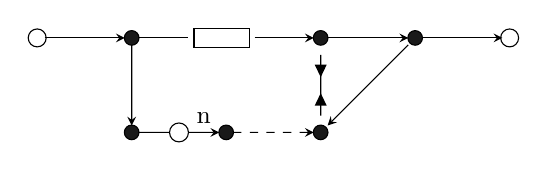
\begin{tikzpicture}[scale=1.2]
  \tikzset{every node} = [font=\small]

  \ionode{(P-A)}{(0,0)}{}
  \ionode{(P-B)}{(5,0)}{}
  \mixednode{(P-C)}{(1,0)}{}
  \mixednode{(P-D)}{(3,0)}{}
  \mixednode{(P-E)}{(4,0)}{}
  \mixednode{(P-F)}{(1,-1)}{}
  \mixednode{(P-G)}{(2,-1)}{}
  \mixednode{(P-H)}{(3,-1)}{}

  \fifoe{(P-C)}{(P-D)}{}
  \syncdrain{(P-D)}{(P-H)}{}
  \sync{(P-A)}{(P-C)}{}
  \sync{(P-C)}{(P-F)}{}
  \sync{(P-D)}{(P-E)}{}
  \sync{(P-E)}{(P-B)}{}
  \sync{(P-E)}{(P-H)}{}
  \lossysync{(P-G)}{(P-H)}{}

  \timer{(P-F)}{(P-G)}{node [above] {n}}

\end{tikzpicture}

  \end{center}
  \caption{Expiring FIFO1 Channel (ExpFIFO1)}
  \label{fig:expfifo}
\end{figure}

Informally speaking, an expiring FIFO1 channel with \emph{timeout} $n$ is able to accept a data item
and stored it in the buffer cell for $n$ time units. If a read operation on $B$ is performed within
$n$ time units, it will obtain the data item successfully and clear the buffer. However, the data
item would be dropped if no read operation comes.

\begin{figure}[ht]
  \begin{center}
    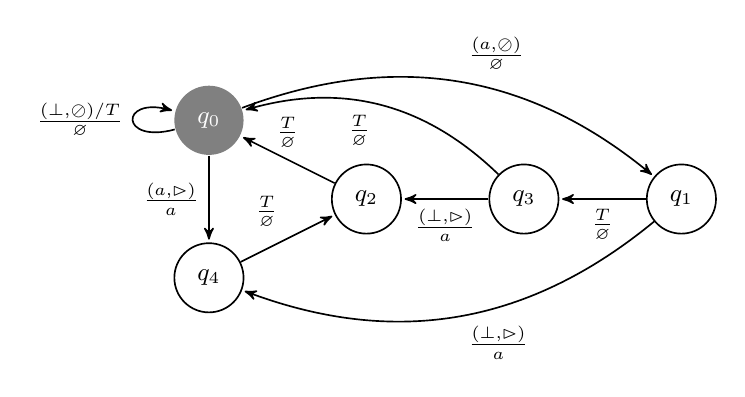
\begin{tikzpicture}[->,>=stealth',shorten >=1pt,auto,node distance=1.9cm,
  semithick]
  \tikzstyle{initial}=[fill=gray,text=white]
  \tikzstyle{every node}=[font=\small]
  \tikzstyle{nodraw}=[draw=none]

  \node[initial,state, nodraw] (Q0) at (0,1)   {$q_0$};
  \node[state]         (Q1) at (6,0)   {$q_1$};
  \node[state]         (Q2) at (2,0)  {$q_2$};
  \node[state]         (Q3) at (4,0)   {$q_3$};
  \node[state]         (Q4) at (0,-1)  {$q_4$};
  
  \path
  (Q0) edge [bend left]  node         {$\frac{(a,\rnoread)}{\rempty}$} (Q1)
  (Q0) edge              node [left]  {$\frac{(a,\rread)}{a}$} (Q4)
  (Q0) edge [loop left]  node         {$\frac{(\bot,\rnoread)/T}{\rempty}$} (Q0)
  (Q1) edge              node         {$\frac{T}{\rempty}$} (Q3)
  (Q1) edge [bend left]  node         {$\frac{(\bot,\rread)}{a}$} (Q4)
  (Q2) edge              node [above] {$\frac{T}{\rempty}$} (Q0)
  (Q3) edge              node         {$\frac{(\bot,\rread)}{a}$} (Q2)
  (Q3) edge [bend right] node         {$\frac{T}{\rempty}$} (Q0)
  (Q4) edge              node         {$\frac{T}{\rempty}$} (Q2)
  ;
\end{tikzpicture}


  \end{center}
  \caption{Learn Result of The ExpFIFO1 where $n=2,\Sigma=\{a\}$}
  \label{fig:expfifosemantics}
\end{figure}

Figure \ref{fig:expfifosemantics} shows the learning result of this example.
To simplify the graph, we ignore the all the trivial transitions $\frac{\bot,\rnoread}{\rempty}$
and block transitions. More details of this case can be found in our \emph{github repo}.

\subsection{Performance Optimization}
As a well-known learning algorithm, L* has proved its efficiency in models without time.
However, when dealing with timed connectors, the algorithm failed to meet our expectation.

\begin{table}[ht]
  \renewcommand{\arraystretch}{1.3}
  \caption{Time-Cost Analysis}
  \label{tabel:timecost}
  \centering
  \begin{tabular}{l||rrr}
    \hline
    & FIFO & Alternator & Gate \\
    \hline\hline
    Membership Query(s) & 41.571 & 126.468 & 169.161 \\
    Hypothesis Query(s) & 0.001 & 0.003 & 0.004 \\
    Total Time(s) & 41.715 & 165.114 & 247.098 \\
    Membership Query(\%) & 99.6 & 76.6 & 68.5 \\
    \hline
  \end{tabular}
\end{table}

As shown in Table \ref{tabel:timecost}, time consumption mainly comes from membership queries.
With time involved, every single membership query takes a lot of time inevitably.
After reviewing our algorithm, we found that simulations on similar sequences were invoked frequently:

\begin{itemize}
  \item When constructing \emph{Obs} tables, there are lots of redundant calls to membership
    queries. For example, a sequence with prefix 'aa' and suffix 'b' is exactly same as another one
    with prefix 'a' and suffix 'ab'.
  \item Simulation on mealy machines can provide multi-step output. Consequently, if we have
    simulated an 'abc' sequence, there's no reason to perform simulation on an 'ab' sequence.
\end{itemize}

If previous simulation results are stored in a well-maintained cache, the time-cost in
simulation process could be reduced signficiantly. In this work, we use a multiway tree to buffer
these results.

\begin{table}[ht]
  \renewcommand{\arraystretch}{1.3}
  \caption{Reduction of Membership Queries}
  \label{tabel:cacheoptimization}
  \centering
  \begin{tabular}{l||rrr}
    \hline
    & FIFO & Alternator & Gate \\
    \hline\hline
    Original Algorithm & 93 & 880 & 1034 \\
    Cached Algorithm & 90 & 725 & 707 \\
    Reduction Rate & 3.2\% & 21.4\% & 31.6\% \\
    \hline
  \end{tabular}
\end{table}

With cache applied, we have made considerable reduction on the calls of membership queries. The results
can be found in Table \ref{tabel:cacheoptimization}.

\subsection{An Example of the Reo Package }
\label{sec:reolib}

Our implementation in \texttt{Golang} is well-prepared not only for academic use
but also for practical concurrent programming. The following code shows how to compose an alternator
connector (see in Figure \ref{fig:reoconnector}) in \texttt{Golang}. An intact version of this example
can be found in our github repo.

\begin{lstlisting}
func alternator(A, B, C Port) {
  M := MakePorts(6)

  // definition of channels
  go ReplicatorChannel(A, M[0], M[1])
  go ReplicatorChannel(B, M[2], M[3])
  go MergerChannel(M[4], M[5], C)

  go SyncdrainChannel(M[1], M[2])
  go SyncChannel(M[0], M[4])
  go FifoChannel(M[3], M[5])
}
\end{lstlisting}

Provided with the source and sink nodes, \emph{alternator} function creates a series of basic
channels and mixed nodes (named \emph{Port}) to serve as the alternator connector we need. Now we
can activate the components and using \emph{alternator} function to coordinate them.

\begin{lstlisting}
A,B,C := MakePorts(3)
alternator(A, B, C)

go sender(A, "MSG A")
go sender(B, "MSG B")
go monitor(C)
\end{lstlisting}

In this case, \emph{sender} are goroutines (basic parallel units in \texttt{Golang}) that keep
sending certain messages to some given port (A and B). A \emph{monitor} keep trying to read data
items from the sink end C and print them on the screen. Finally, we have an interleaved sequence of
``MSG\_A'' and ``MSG\_B''.
 
\section{Conclusion and Future Work}
In this paper, we come up with an approach to extract timed connectors from blackbox
implementations. We propose \emph{parameterized Mealy machine} to describe the behavior of Reo
connectors. Then we define the product operator and link operator, which can be used to
construct complex connectors from simpler ones.
Besides, we show how PMMs behave as the bridge between Reo connectors and concrete Mealy
machines with timed action T provided. 

We also adapt the well-knwon active learning algorithm L* to deal with time domain.
When time is taken into consideration, the original L* algorithm run into the bottleneck.
By a tree-style cache, we make significant reduction on membership queries and, in turn,
improve the performance of learning algorithm. As a by-product, we also encapsulate the Reo
connector as a distributable package which could contribute to concurrent programming.

Our future works would mainly focus on better support of dense time. To describe dense
time behavior, the Mealy machine model needs a lot of changes instead of a simple T action. Besides,
we will also try to improve our algorithm to handle non-deterministic behaviors. This is not a brand
new topic \cite{DBLP:conf/isola/VolpatoT14}, but we believe that there is still room for
improvement.  

\section*{Acknowledgments}
The work was partially supported by the National Natural Science Foundation of China under grant no.
61202069, 61272160 and 61532019, and Research Fund for the Doctoral Program of Higher Education of
China under grant no. 20120001120103.

\bibliographystyle{abbrv}
\bibliography{bib}

\end{document}
